\documentclass[a4paper,10pt,openany]{article}

\usepackage[bitstream-charter]{mathdesign}
\usepackage{libertine}

\usepackage[left=19mm,right=19mm, top=2.5cm, bottom=2.9cm]{geometry}


% for proper Encoding
\usepackage[utf8]{inputenc}
\usepackage[english]{babel}

%Mathesatz
\usepackage{amsmath}
%\usepackage{amssymb}

%fancy looks:
\usepackage{microtype}

%for clickable references, much nicer to read
\usepackage{hyperref}

%for references with page numbers
\usepackage[english,vario]{fancyref}
\vrefwarning


\usepackage{graphicx}

\parindent 0pt %remove indentation for a new paragraph


%title, author
\title{The RK2 methods}
\author{Dan Čermák}
%\date{\today}

\begin{document}

\maketitle

\section{Introduction}

The RK2 methods can be used to solve differential equations of the form:
\begin{equation}
\dot{y} = f(y, t)
\end{equation}

As we are interested in the application on gravity, we will drop the time dependence as it is not present.

There are actually two major RK2 methods in contrast to fourth order Runge-Kutta where there is \textbf{the} RK4 method.

The first method is the so called mid-point method:
\begin{equation}
 y_{n+1} = y_n + hf\left( y_n+\frac{h}{2}f( y_n) \right)
\end{equation}

The second method is the method from the script, also called Heun's method:
\begin{equation}
y_{n+1} = y_{n} + \frac{h}{2} \left( f( y_n) + f(y_n + h f(y_n)) \right)
\end{equation}

Both methods are nearly equivalent, but they perform differently.


\section{Application}

For the n-body problem we can construct the following ODE:
\begin{equation}
y = \begin{pmatrix} \mathbf{x}\\ \mathbf{v} \end{pmatrix} \text{ where: }\dot{y} = \begin{pmatrix} \mathbf{v}\\ \mathbf{a} \end{pmatrix}
\end{equation}
where $\mathbf{x}$ is the position, $\mathbf{v}$ the velocity and $\mathbf{a}$ the acceleration given by Newton's law.

In the following we will apply this to Heun's method:

\begin{align}
f(y_n) = f \begin{pmatrix} \mathbf{x_n}\\ \mathbf{v_n} \end{pmatrix} = \begin{pmatrix} \mathbf{v_n}\\ \mathbf{a_n} \end{pmatrix}\\
f(y_n + h f(y_n) ) = f \begin{pmatrix} \mathbf{x_n} + h\mathbf{v_n} \\ \mathbf{v_n} + h \mathbf{a_n} \end{pmatrix} = \begin{pmatrix}  \mathbf{v_n} + h \mathbf{a_n} \\ \mathbf{a} (\mathbf{x_n} + h\mathbf{v_n}) \\ \end{pmatrix}
\end{align}
where $\mathbf{a} (\mathbf{x_n} + h\mathbf{v_n})$ is the acceleration at $\mathbf{x_n} + h\mathbf{v_n}$.

This results in the following formulas for $\mathbf{x_{n+1}}$ and  $\mathbf{v_{n+1}}$:
\begin{align}
\mathbf{x_{n+1}} &= \mathbf{x_n} +  h\mathbf{v_n} +  \frac{h}{2} \mathbf{a_n}\\
\mathbf{v_{n+1}} &= \mathbf{v_n} +  \frac{h}{2} \mathbf{a_n} + \frac{h}{2} \mathbf{a} (\mathbf{x_n} + h\mathbf{v_n})
\end{align}



\begin{figure}
\begin{center}
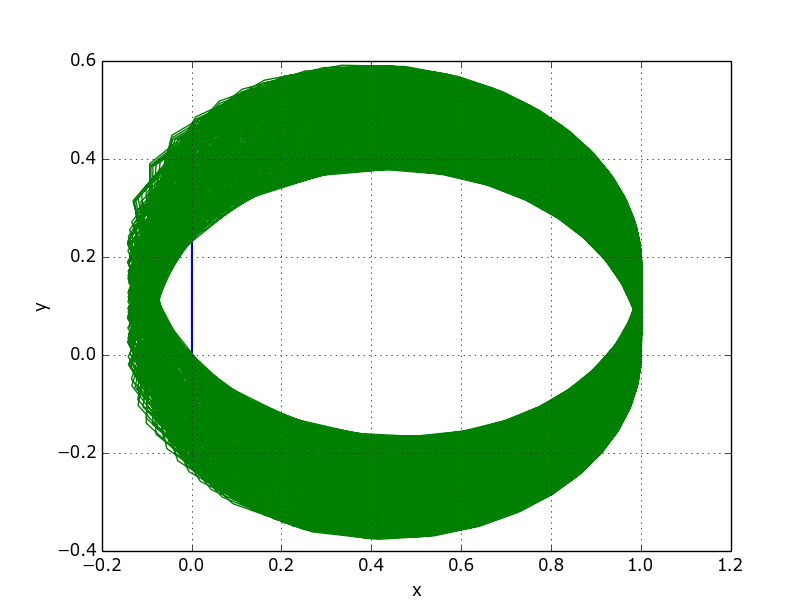
\includegraphics[width=.7\textwidth]{midpoint_pos.png}\\
\end{center}
\begin{center}
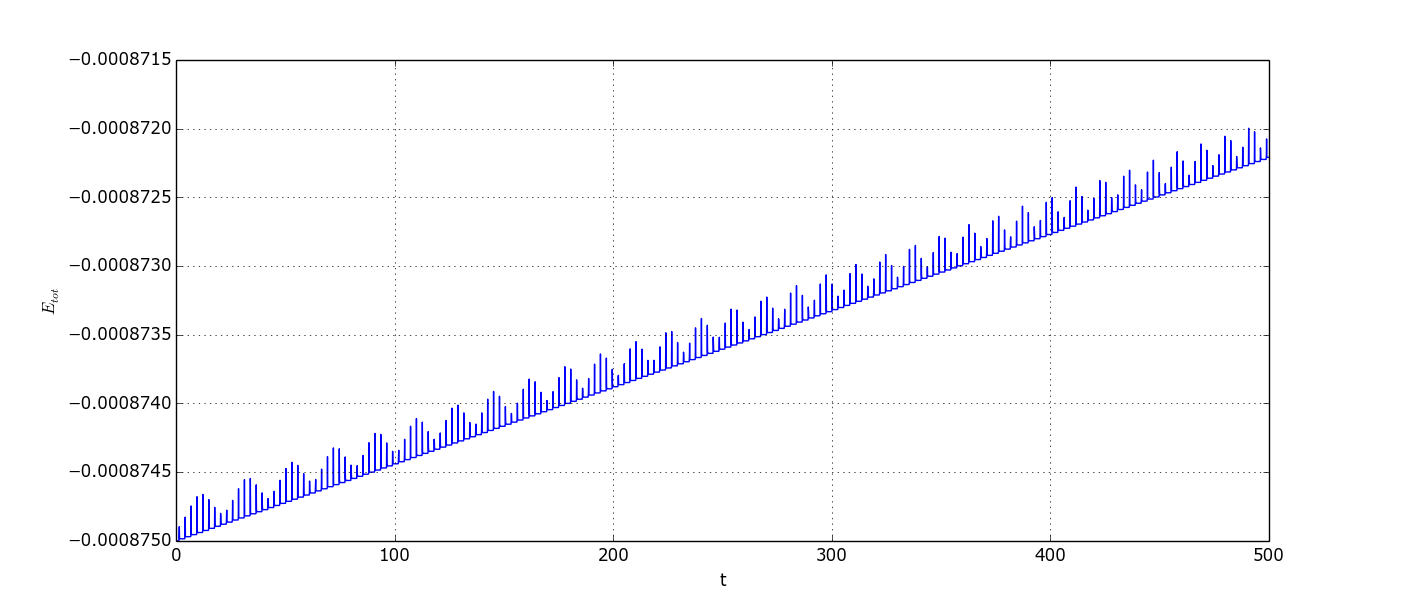
\includegraphics[width=\textwidth]{midpoint_energy.png}\\
\end{center}
\caption{Example simulation of the two body problem with the midpoint method with small time steps. The upper image shows the position of both bodies, the lower the total energy.}\label{fig:midpoint performance}
\end{figure}

Surprisingly, Heun's method performs poorly in the two body problem (as you have all seen). Even for very small time steps you will get a decaying orbit. This is not the case for the midpoint method! For small time steps (so small that he leapfrog's numerical perihelion shift is barely noticeable) the orbit decay is very small, though the energy is obviously not bound as you can see in \fref{fig:midpoint performance}.


 
\end{document}